\documentclass[11pt,a4paper]{article}
\usepackage[T1]{fontenc}
\usepackage[utf8]{inputenc}
\usepackage[spanish,english,es-noshorthands]{babel}
\usepackage[margin=2cm]{geometry}
\usepackage{amsmath,booktabs,graphicx,float,url}
\title{Supplementary Material: Expressed Affective Polarization in YouTube Comments}
\author{}
\date{November 22, 2026}
\begin{document}\maketitle
This material expanded the observational study's tables and diagnostics. Measurement units were comparable users for affective polarization and comment--target pairs for classifier evaluation. Complementary analyses were defined after the primary result to examine scope and stability rather than to select specifications by significance. This edition concerned 300 examined histories and the five-model evaluation, with additional diagnostics for the three original references.
\section{Selection and measurement evidence}
The 4\,443 structural candidates were not already comparable users. Of the first 300 examined in the fixed order, 174 failed affinity requirements, 126 met them, and 122 also qualified in B. Among the four remaining exclusions, one lacked ingroup evidence, two lacked outgroup evidence, and one had insufficient B events. This hierarchy gave mutually exclusive reasons; one outgroup absence also coincided with insufficient events. Early exclusions based on the affinity criteria left 709 comments unread in 56 excluded histories, rather than annotating them as target absence. Comparable-user histories were read completely.

Videos were assigned by hash with seed 42 to disjoint sets A (affinity assignment) and B (evaluation); the sets were not chronological periods. Reading started with A, ordering videos by size and breaking ties by identifier. Remaining comments were skipped only when a conservative bound proved that neither bloc could meet the affinity requirements, even if every unread comment was counted as possible support. Skipped observations remained missing rather than being labeled as target absence. Users meeting the affinity criteria required complete reading of both A and B.

The shared training recipe used seeds 42, 43, and 44, AdamW with learning rate $2\times10^{-5}$, weight decay 0.01, effective batch size 16, at most eight epochs, and early stopping after two epochs without validation improvement. These settings remained fixed in the encoder extension. Probabilities were averaged across the three seeds before calibration on validation data.



Table~\ref{tab:supp_selection} compared observable participation between included and excluded users.

\begin{table}[H]\centering\small
\caption{Observable participation by inclusion status.}
\label{tab:supp_selection}
\setlength{\tabcolsep}{4pt}
\begin{tabular}{lrrr}\toprule
Variable & Included (122) & Excluded (178) & SMD\\\midrule
Comments & 33.50 [20.00, 60.00] & 28.00 [16.25, 51.75] & 0.271\\
Videos & 24.00 [16.00, 40.75] & 21.00 [13.25, 32.75] & 0.225\\
Channels & 7.00 [5.00, 9.00] & 6.00 [4.00, 8.00] & 0.271\\
Source groups & 3.00 [2.00, 3.00] & 2.50 [2.00, 3.00] & 0.121\\
\bottomrule\end{tabular}
\par\smallskip\footnotesize Values were median [25th, 75th percentile]. SMD: standardized mean difference.
\end{table}

Positive SMDs indicated greater mean activity among comparable users. These described observable selection; they neither corrected unobserved differences nor justified generalization to all YouTube users.

Table~\ref{tab:supp_robust} summarized the location, dispersion, and event support of individual measurements.

\begin{table}[H]\centering\small
\caption{Summary statistics for comparable users.}
\label{tab:supp_robust}
\setlength{\tabcolsep}{4pt}
\begin{tabular}{lrrrrr}\toprule
Metric & Mean & SD & Median & IQR & 10\% trimmed mean\\\midrule
$\mathrm{AP}_{In}$ & 3.328 & 8.609 & 2.000 & [1.000, 4.000] & 2.541\\
$\mathrm{AP}_{Out}$ & -6.090 & 9.600 & -3.000 & [-5.750, -2.000] & -4.000\\
AP & 9.418 & 14.296 & 6.000 & [4.000, 10.000] & 6.837\\
Dispersion & 2.010 & 1.156 & 1.789 & [1.414, 2.236] & 1.817\\
Normalized gap & 1.442 & 0.547 & 1.600 & [1.000, 2.000] & 1.511\\
Ingroup events & 6.230 & 10.980 & 4.000 & [3.000, 7.000] & 4.347\\
Outgroup events & 6.959 & 10.130 & 4.000 & [2.000, 6.000] & 4.755\\
B events & 13.189 & 18.749 & 8.000 & [5.000, 13.000] & 9.347\\
B videos & 8.025 & 7.932 & 6.000 & [4.000, 9.750] & 6.520\\
\bottomrule\end{tabular}
\par\smallskip\footnotesize SD: standard deviation. IQR was reported as [25th, 75th percentile]. The trimmed mean removed 10\% of observations from each tail.
\end{table}

Normalization and equal contribution per user reduced the influence of high activity on the aggregate contrast. They did not remove uncertainty in short histories. Median support of eight B events and six B videos was therefore relevant to the interpretation of individual scores.

Table~\ref{tab:supp_composition} reported how evaluations were distributed across partitions and political destinations.

\begin{table}[H]\centering\small
\caption{Comment--bloc events by partition, affinity, target, and evaluation.}
\label{tab:supp_composition}
\setlength{\tabcolsep}{4pt}
\begin{tabular}{lrrrrrrr}\toprule
Partition & Affinity & Target & Fav. & Unfav. & Neutral & Mixed & Not eval.\\\midrule
A & Right & Right & 314 & 84 & 84 & 11 & 2\\
A & Right & Left & 2 & 277 & 30 & 0 & 1\\
A & Left & Right & 2 & 504 & 41 & 3 & 4\\
A & Left & Left & 290 & 61 & 64 & 5 & 0\\
B & Right & Right & 239 & 42 & 91 & 11 & 1\\
B & Right & Left & 2 & 233 & 32 & 1 & 2\\
B & Left & Right & 5 & 517 & 60 & 4 & 3\\
B & Left & Left & 273 & 64 & 51 & 13 & 1\\
\bottomrule\end{tabular}
\par\smallskip\footnotesize Mixed and not-evaluable events did not contribute to balances. Counts were events, not independent people.
\end{table}

\section{Sensitivity of the normalized gap}

Table~\ref{tab:supp_sensitivity} compared the original sensitivity variants with the primary definition on matched users.

\begin{table}[H]\centering\small
\caption{Original sensitivity variants and matched comparisons.}
\label{tab:supp_sensitivity}
\setlength{\tabcolsep}{4pt}
\begin{tabular}{lrrrrr}\toprule
Variant & Users & Gap & 95\% CI & Original & Change CI\\\midrule
Reversed A/B & 76 & 1.520 & [1.227, 1.674] & 1.581 & [-0.212, 0.125]\\
Video-balanced & 122 & 1.473 & [1.284, 1.698] & 1.442 & [-0.047, 0.081]\\
Without Keiko Fujimori & 80 & 1.505 & [1.238, 1.709] & 1.467 & [-0.062, 0.147]\\
Without Roberto Sánchez & 90 & 1.447 & [1.294, 1.684] & 1.437 & [-0.070, 0.082]\\
Without Rafael López Aliaga & 98 & 1.506 & [1.318, 1.717] & 1.506 & [-0.020, 0.039]\\
Historical data only & 100 & 1.493 & [1.308, 1.755] & 1.504 & [-0.054, 0.049]\\
\bottomrule\end{tabular}
\par\smallskip\footnotesize Original: primary gap restricted to the retained users. Change CI: 95\% interval for the paired change.
\end{table}

Changes in retained population and changes in measurement were distinct. Comparing variants with the original definition on the same users avoided attributing selection differences to the formula. No paired-change interval for these six variants excluded zero; this did not demonstrate equivalence.

Table~\ref{tab:supp_grid} reported retention and normalized gaps across the fixed threshold grid.

\begin{table}[H]\centering\small
\caption{Fixed grid of event-support and affinity criteria.}
\label{tab:supp_grid}
\setlength{\tabcolsep}{4pt}
\begin{tabular}{lrrr}\toprule
Criterion & Users & Gap & 95\% CI\\\midrule
e=2, s=2/3, p=2 & 123 & 1.431 & [1.281, 1.653]\\
e=2, s=2/3, p=3 & 81 & 1.468 & [1.279, 1.671]\\
e=2, s=3/4, p=2 & 121 & 1.445 & [1.287, 1.661]\\
e=2, s=3/4, p=3 & 80 & 1.481 & [1.285, 1.675]\\
e=3, s=2/3, p=2 & 122 & 1.442 & [1.276, 1.682]\\
e=3, s=2/3, p=3 & 80 & 1.486 & [1.278, 1.692]\\
e=3, s=3/4, p=2 & 120 & 1.457 & [1.281, 1.688]\\
e=3, s=3/4, p=3 & 79 & 1.500 & [1.280, 1.699]\\
e=5, s=2/3, p=2 & 98 & 1.476 & [1.285, 1.708]\\
e=5, s=2/3, p=3 & 67 & 1.501 & [1.280, 1.715]\\
e=5, s=3/4, p=2 & 96 & 1.494 & [1.292, 1.718]\\
e=5, s=3/4, p=3 & 66 & 1.518 & [1.288, 1.721]\\
\bottomrule\end{tabular}
\par\smallskip\footnotesize e: minimum B events; s: dominant positive share in A; p: minimum A positives. Two positive A videos remain required.
\end{table}

The grid resampled the 300 examined users and allowed relaxed criteria to admit users with complete histories. Early exclusions received no imputed labels. Consequently, the original-threshold row could have a slightly different interval from the bootstrap conditional on the 122 original comparables. Changes in the grid reflected retention because the individual scoring formula remained fixed.

Table~\ref{tab:supp_support} reported the additional support, denominator, and source-specific checks.

\begin{table}[H]\centering\small
\caption{Event support, neutral denominators, and source provenance.}
\label{tab:supp_support}
\setlength{\tabcolsep}{4pt}
\begin{tabular}{lrrr}\toprule
Variant & Users & Gap & 95\% CI\\\midrule
Events per bloc: 1 & 122 & 1.442 & [1.273, 1.683]\\
Events per bloc: 2 & 95 & 1.418 & [1.248, 1.683]\\
Events per bloc: 3 & 66 & 1.406 & [1.203, 1.671]\\
Events per bloc: 5 & 30 & 1.395 & [1.091, 1.683]\\
Without neutral denominators & 114 & 1.669 & [1.507, 1.885]\\
Left sources & 63 & 1.497 & [1.188, 1.788]\\
Right sources & 16 & 1.381 & [0.785, 1.921]\\
Neutral sources & 52 & 1.468 & [1.079, 1.777]\\
\bottomrule\end{tabular}
\par\smallskip\footnotesize Source-specific subsets could overlap and required both target blocs within each subset.
\end{table}

Requiring five events per bloc retained 30 users and widened uncertainty. Removing neutral events from denominators retained 114: the gap rose from 1.4827 to 1.6687 on those same users, a change of 0.1859 [0.0897, 0.2883]. The primary definition preserved neutral evidence and moderated magnitude. Eight users lost positive denominators in the variant. Mixed events had already been excluded; removing them again did not constitute an additional sensitivity analysis.

\section{Individual stability and adverse errors}
Among 113 users measurable in A and B, the mean A gap was 1.5810 and the mean B gap 1.4152. A minus B was 0.1658, 95\% CI [$-0.0494$, 0.3290]. The point estimate was compatible with optimism from reusing A, but the interval did not demonstrate inflation. Separating A/B was justified by design rather than by obtaining this contrast.

The 200 random B-video splits retained A affinity, required two events and both blocs in each half, and compared only users measurable in both. They retained 51--74 users (median 63). Median Pearson correlation was 0.3667, IQR [0.3032, 0.4203]; median Spearman correlation was 0.3806, IQR [0.3272, 0.4448]. These described variation across partitions, not confidence intervals or population reliability. The aggregate direction was more stable than individual ordering \cite{Pronk2022SplitHalf}.


Table~\ref{tab:supp_adverse} reported the conditional worst-case gap under each error budget.

\begin{table}[H]\centering\small
\caption{Worst-case gap after changing a budget of B evaluations.}
\label{tab:supp_adverse}
\setlength{\tabcolsep}{4pt}
\begin{tabular}{lrr}\toprule
Budget & Changed events & Minimum gap\\\midrule
0\% & 0 & 1.442\\
5\% & 80 & 0.639\\
10\% & 160 & 0.180\\
20\% & 321 & -0.541\\
\bottomrule\end{tabular}
\par\smallskip\footnotesize Affinity, users, targets, and denominators remained fixed.
\end{table}

Events with the largest influence were changed first toward ingroup rejection or outgroup support. The mean became nonpositive after 193 of 1\,609 directed changes (12.00\%). This deterministic conditional bound neither estimated actual error frequency nor included errors in A, extraction, unknown targets, or selection. A global classifier confusion matrix was not transferred to histories because their distributions and abstention differed \cite{Egami2023Surrogates}.

\section{Five-model evaluation and accepted predictions}

This section included RoBERTuito, BETO, XLM-RoBERTa, MrBERT-es, and mDeBERTa-v3-base on the same 3,000-comment evaluation sample. The integral union had 5,165 pairs; the common complete-context panel had 3,222. Sampling weights were retained. F1 was measured before abstention; accepted precision and coverage used the original validation calibration without refitting on this sample.

Table~\ref{tab:supp_five_models} reported the five models' end-to-end performance and accepted predictions.

\begin{table}[H]\centering\small
\caption{Five-model end-to-end results and video-bootstrap uncertainty.}
\label{tab:supp_five_models}
\setlength{\tabcolsep}{4pt}
\begin{tabular}{lrrr}\toprule
Model & Metric & Estimate & 95\% CI\\\midrule
RoBERTuito & Macro-F1 & 0.384 & [0.358, 0.412]\\
RoBERTuito & Coverage (\%) & 10.328 & [9.146, 11.823]\\
RoBERTuito & Favorable precision & 0.808 & [0.768, 0.847]\\
RoBERTuito & Unfavorable precision & 0.868 & [0.832, 0.904]\\
BETO & Macro-F1 & 0.324 & [0.301, 0.348]\\
BETO & Coverage (\%) & 21.206 & [19.111, 23.723]\\
BETO & Favorable precision & 0.798 & [0.751, 0.843]\\
BETO & Unfavorable precision & 0.733 & [0.706, 0.759]\\
XLM-RoBERTa & Macro-F1 & 0.283 & [0.262, 0.306]\\
XLM-RoBERTa & Coverage (\%) & 3.324 & [2.781, 3.944]\\
XLM-RoBERTa & Favorable precision & 0.793 & [0.743, 0.845]\\
XLM-RoBERTa & Unfavorable precision & --- & [---, ---]\\
MrBERT-es & Macro-F1 & 0.323 & [0.301, 0.346]\\
MrBERT-es & Coverage (\%) & 10.084 & [8.860, 11.492]\\
MrBERT-es & Favorable precision & 0.737 & [0.693, 0.781]\\
MrBERT-es & Unfavorable precision & 0.836 & [0.793, 0.875]\\
mDeBERTa-v3-base & Macro-F1 & 0.309 & [0.287, 0.332]\\
mDeBERTa-v3-base & Coverage (\%) & 3.193 & [2.676, 3.822]\\
mDeBERTa-v3-base & Favorable precision & 0.831 & [0.779, 0.879]\\
mDeBERTa-v3-base & Unfavorable precision & --- & [---, ---]\\
\bottomrule\end{tabular}
\par\smallskip\footnotesize Intervals used 2,000 video-bootstrap replicates. Coverage was the accepted share of evaluable target weight. A dash indicated no accepted predictions or insufficient support, not zero precision.
\end{table}

Table~\ref{tab:supp_common} reported classification conditional on the shared complete-context inputs.

\begin{table}[H]\centering\small
\caption{Common complete-context candidates: classification and accepted share.}
\label{tab:supp_common}
\setlength{\tabcolsep}{4pt}
\begin{tabular}{lrrr}\toprule
Model & Macro-F1 & 95\% CI & Coverage (\%)\\\midrule
RoBERTuito & 0.5979 & [0.5771, 0.6174] & 26.17\\
BETO & 0.4993 & [0.4814, 0.5173] & 47.26\\
XLM-RoBERTa & 0.4309 & [0.4143, 0.4477] & 8.27\\
MrBERT-es & 0.5025 & [0.4838, 0.5202] & 24.06\\
mDeBERTa-v3-base & 0.4733 & [0.4564, 0.4905] & 8.05\\
\bottomrule\end{tabular}
\par\smallskip\footnotesize Conditional results excluded extraction omissions and were not end-to-end coverage. The same video resampling design was used for the macro-F1 intervals.
\end{table}

RoBERTuito retained the largest end-to-end macro-F1. BETO and MrBERT-es showed no clear difference in that metric, without establishing equivalence. MrBERT-es accepted favorable and unfavorable predictions; mDeBERTa accepted favorable only. Neither new model enabled neutral predictions under the stored calibration. Validation precision thresholds were selection rules and did not guarantee the same precision on this evaluation sample.

The following historical diagnostics retained their original three-reference scope; their confusion matrices, seed variability, loss decomposition, and confidence curves were not presented as five-model results.

\section{Reference-classifier diagnostics}

These diagnostics concerned only the evaluated RoBERTuito, BETO, and XLM-RoBERTa references. The weighted training-majority class was unfavorable: predicting it for available candidates while preserving omissions yielded end-to-end macro-F1 0.1524. This was neither calibrated coverage nor an independent reference. All three models outperformed its F1, but their results did not justify automatic measurement across the full collection \cite{GrimmerStewart2013}.

Table~\ref{tab:supp_classes} located class-specific errors before confidence selection.

\begin{table}[H]\centering\small
\caption{Per-class performance before abstention, including omissions.}
\label{tab:supp_classes}
\setlength{\tabcolsep}{4pt}
\begin{tabular}{lrrrrr}\toprule
Model & Class & Precision & Recall & F1 & Pairs\\\midrule
RoBERTuito & Favorable & 0.680 & 0.359 & 0.470 & 858\\
RoBERTuito & Unfavorable & 0.690 & 0.338 & 0.454 & 3099\\
RoBERTuito & Neutral & 0.463 & 0.151 & 0.227 & 992\\
RoBERTuito & Mixed & 0.589 & 0.026 & 0.050 & 39\\
RoBERTuito & Not evaluable & 0.244 & 0.040 & 0.068 & 177\\
BETO & Favorable & 0.551 & 0.363 & 0.438 & 858\\
BETO & Unfavorable & 0.649 & 0.346 & 0.451 & 3099\\
BETO & Neutral & 0.516 & 0.045 & 0.082 & 992\\
BETO & Mixed & 0.000 & 0.000 & 0.000 & 39\\
BETO & Not evaluable & 0.198 & 0.014 & 0.026 & 177\\
XLM-RoBERTa & Favorable & 0.529 & 0.295 & 0.379 & 858\\
XLM-RoBERTa & Unfavorable & 0.623 & 0.361 & 0.457 & 3099\\
XLM-RoBERTa & Neutral & 0.474 & 0.007 & 0.014 & 992\\
XLM-RoBERTa & Mixed & 0.000 & 0.000 & 0.000 & 39\\
XLM-RoBERTa & Not evaluable & 0.000 & 0.000 & 0.000 & 177\\
\bottomrule\end{tabular}
\par\smallskip\footnotesize Metrics used sampling weights; support was the raw number of pairs.
\end{table}

Primary macro-F1 averaged favorable, unfavorable, and neutral. Mixed and not evaluable were shown to locate errors without changing that definition. Neutral had particularly low F1 and was disabled by original calibration in all references, as were mixed and not evaluable. RoBERTuito and BETO accepted favorable and unfavorable predictions; XLM-RoBERTa accepted favorable only. Acceptance required weighted validation precision of at least 0.85 and at least ten accepted comment--target pairs per class. Both values were study-defined heuristics: the precision target prioritized reliability among retained predictions, and the count requirement avoided enabling a class on very few cases. Ten referred to the raw number of accepted pairs, without adjustment for sampling weights or dependence within comments or videos; it did not establish statistical sufficiency. These criteria did not provide an out-of-sample precision guarantee. Selective classification motivated the error--coverage tradeoff \cite{Geifman2017Selective}, and temperature scaling supplied the probability-calibration method \cite{Guo2017Calibration}; neither reference prescribed these numerical values. Evaluation-sample results did not modify the stored acceptance rules.

Table~\ref{tab:supp_seeds} reported between-seed variability on validation data.

\begin{table}[H]\centering\small
\caption{Weighted validation macro-F1 across three training seeds.}
\label{tab:supp_seeds}
\setlength{\tabcolsep}{4pt}
\begin{tabular}{lrrr}\toprule
Model & Seeds & Mean & SD\\\midrule
RoBERTuito & 3 & 0.6024 & 0.0559\\
BETO & 3 & 0.4979 & 0.0564\\
XLM-RoBERTa & 3 & 0.4494 & 0.0973\\
\bottomrule\end{tabular}
\par\smallskip\footnotesize SD: standard deviation between fits. These were validation scores, not repeated independent evaluation samples.
\end{table}

The ensemble averaged probabilities, so its F1 was not the mean of per-seed F1. BERTIN remained in historical files only, outside the active comparison.

Table~\ref{tab:supp_confusion} reported the weighted confusion patterns within each reference class.

\begin{table}[H]\centering\small
\caption{Confusion matrices: weighted percentages within reference rows.}
\label{tab:supp_confusion}
\setlength{\tabcolsep}{4pt}
\begin{tabular}{lrrrrrrr}\toprule
Model & Reference & F & U & N & M & NE & O\\\midrule
RoBERTuito & Favorable & 35.9 & 17.7 & 5.7 & 0.0 & 0.0 & 40.7\\
RoBERTuito & Unfavorable & 2.0 & 33.8 & 3.1 & 0.0 & 0.2 & 60.9\\
RoBERTuito & Neutral & 4.2 & 28.9 & 15.1 & 0.1 & 0.9 & 50.9\\
RoBERTuito & Mixed & 7.9 & 32.0 & 6.6 & 2.6 & 0.0 & 50.9\\
RoBERTuito & Not evaluable & 14.0 & 61.8 & 15.5 & 0.0 & 4.0 & 4.7\\
BETO & Favorable & 36.3 & 21.3 & 1.5 & 0.0 & 0.1 & 40.7\\
BETO & Unfavorable & 3.7 & 34.6 & 0.7 & 0.0 & 0.2 & 60.9\\
BETO & Neutral & 7.9 & 36.7 & 4.5 & 0.0 & 0.0 & 50.9\\
BETO & Mixed & 10.6 & 35.9 & 2.6 & 0.0 & 0.0 & 50.9\\
BETO & Not evaluable & 18.4 & 72.0 & 3.5 & 0.0 & 1.4 & 4.7\\
XLM-RoBERTa & Favorable & 29.5 & 29.4 & 0.3 & 0.0 & 0.0 & 40.7\\
XLM-RoBERTa & Unfavorable & 2.9 & 36.1 & 0.1 & 0.0 & 0.0 & 60.9\\
XLM-RoBERTa & Neutral & 7.7 & 40.7 & 0.7 & 0.0 & 0.0 & 50.9\\
XLM-RoBERTa & Mixed & 4.0 & 45.1 & 0.0 & 0.0 & 0.0 & 50.9\\
XLM-RoBERTa & Not evaluable & 22.0 & 72.6 & 0.6 & 0.0 & 0.0 & 4.7\\
\bottomrule\end{tabular}
\par\smallskip\footnotesize Predictions: favorable (F), unfavorable (U), neutral (N), mixed (M), not evaluable (NE), omitted (O).
\end{table}

\subsection*{Coverage losses and confidence ordering}

Table~\ref{tab:supp_coverage} separated losses from extraction, incomplete context, and abstention.

\begin{table}[H]\centering\small
\caption{Coverage decomposition over all evaluable target weight.}
\label{tab:supp_coverage}
\setlength{\tabcolsep}{4pt}
\begin{tabular}{lrrrr}\toprule
Model & Omitted & Incomplete context & Abstained & Accepted\\\midrule
RoBERTuito & 55.93 & 4.60 & 29.14 & 10.33\\
BETO & 55.93 & 0.72 & 22.15 & 21.21\\
XLM-RoBERTa & 55.93 & 0.93 & 39.82 & 3.32\\
\bottomrule\end{tabular}
\par\smallskip\footnotesize Percentages summed to 100 within each model.
\end{table}

Recall across all targets, including unknown-bloc actors, was 44.53\%. By actor bloc, recall was 86.36\% for right, 82.09\% for left, and 22.76\% for unknown. Unknown bloc and omitted mention were distinct: some unknown actors were extracted and some known actors omitted. For evaluable targets, the extraction ceiling was 44.07\%; requiring complete context reduced RoBERTuito\textquotesingle s ceiling to 39.47\%. Thus 40\% end-to-end coverage was unattainable for that reference with the current inputs.

\begin{figure}[H]\centering
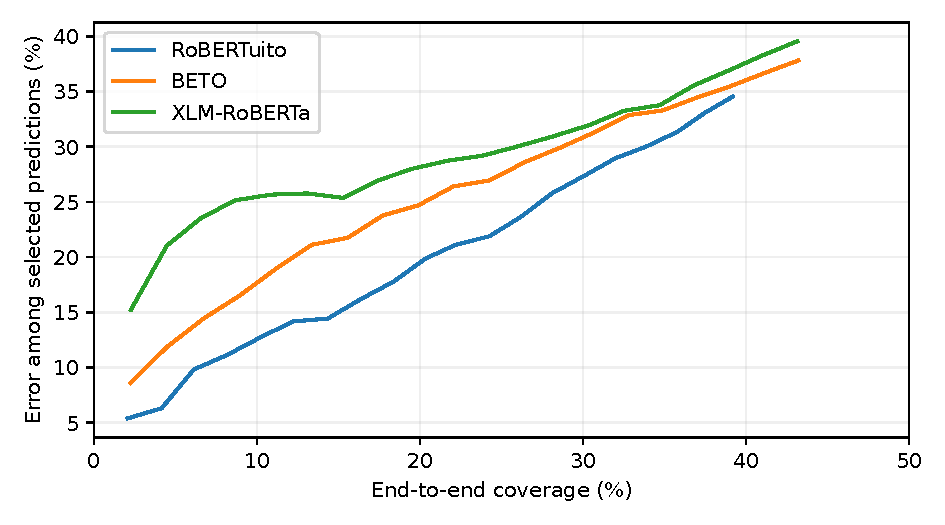
\includegraphics[width=0.9\textwidth]{docs/figures/observational_risk_coverage.pdf}
\caption{Weighted error among selected predictions versus end-to-end coverage when candidates were ranked by confidence. This was a diagnostic, not operational threshold recalibration.}\label{fig:supp_risk_coverage}\end{figure}
Figure~\ref{fig:supp_risk_coverage} illustrated the error--coverage tradeoff. Confidence could not recover absent targets: accepting all candidates still left substantial coverage losses. These curves examined quality and reach together, without choosing a new threshold based on favorable evaluation performance.
\section{Scope and status of this edition}
The limit of 300 examined users was set for resource reasons after annotation progress was known, including 79 comparable users among the first 200. It replaced the original target of 800 comparable users and was not fixed before the study began. The observed gap's 95\% CI half-width was 0.2047, compared with the planned 0.20. The planning target was treated as a precision assumption rather than a universal publication threshold \cite{lakens2022sample}; sampling was not extended in response to the result.

This material accompanied a preprint with provisional results. At the time this version was prepared, history and evaluation annotations remained pending individual human review. Intervals did not include annotation error, and classifier results expressed agreement with initial annotations. Adversarial sensitivity did not replace their confirmation. Model expansion was chosen after examining this sample and was not an independent final evaluation.

Results concerned expressions toward political actors among users with evidence in both blocs. They did not identify the electorate, voting intention, channel causality, or hostility toward every supporter of an opposing bloc. Channel selection, short histories, the registry with 22 documented-bloc identities out of 124, and possible coordinated accounts limited scope. Bots were not identified through a validated procedure. Retrospective capture could not recover deleted content or all original text states. Public tables reported aggregates; identifiers and sensitive affinity inferences required protection and were excluded from figures and tables.
\bibliographystyle{IEEEtran}
\bibliography{docs/references}
\end{document}
